\documentclass[10pt,twocolumn,letterpaper]{article}

\usepackage{cvpr}
\usepackage{times}
\usepackage{epsfig}
\usepackage{graphicx}
\usepackage{amsmath}
\usepackage{amssymb}
\usepackage{gensymb}


% Include other packages here, before hyperref.

% If you comment hyperref and then uncomment it, you should delete
% egpaper.aux before re-running latex.  (Or just hit 'q' on the first latex
% run, let it finish, and you should be clear).
 
\usepackage[pagebackref=true,breaklinks=true,letterpaper=true,colorlinks,bookmarks=true,bookmarksnumbered=true,hypertexnames=false,linkbordercolor={0 0 1}]{hyperref}
% Include other packages here, before hyperref.

% If you comment hyperref and then uncomment it, you should delete
% egpaper.aux before re-running latex.  (Or just hit 'q' on the first latex
% run, let it finish, and you should be clear).
%\usepackage[pagebackref=true,breaklinks=true,letterpaper=true,colorlinks,bookmarks=false]{hyperref}

\cvprfinalcopy % *** Uncomment this line for the final submission

\def\cvprPaperID{****} % *** Enter the CVPR Paper ID here
\def\httilde{\mbox{\tt\raisebox{-.5ex}{\symbol{126}}}}

% Pages are numbered in submission mode, and unnumbered in camera-ready
\ifcvprfinal\pagestyle{empty}\fi
%\setcounter{page}{1}
\begin{document}

%%%%%%%%% TITLE
\title{Dynamical Models for Instruction Completion \\and Error Recognition for NASA Physical Procedures}

\author{Steven Johnson\\
	Department of Computer Sciences\\
	University of Wisconsin--Madison\\
	{\tt\small sjj@cs.wisc.edu}
	\and
	Ronak Mehta\\
	Department of Computer Sciences\\
	University of Wisconsin-Madison\\
	{\tt\small ronakrm@cs.wisc.edu}
	\and
	John Cabaj\\
	Department of Electrical and Computer Engineering\\
	University of Wisconsin-Madison\\
	{\tt\small cabaj@wisc.edu}
}

\maketitle
%\thispagestyle{empty}

%%%%%%%%% ABSTRACT
\begin{abstract}

\end{abstract}

%%%%%%%%% BODY TEXT
\section{Introduction}

Procedures are the accepted means to operate a spacecraft system or systems to perform specific functions, and consequently are at the heart of all NASA human spaceflight operations~\cite{kortenkamp2008procedure}. A procedure is a detailed set of instructions specifying how a piece of equipment is operated or a task is performed~\cite{frank2010plans}. They are often written to be very general and to cover numerous contingencies. Procedures to operate a class of equipment (e.g., smoke detector) will differ based on make, while procedures to operate a piece of equipment will have conditional or optional steps based on configuration. As an additional complication, constraints of some procedures may be highly conditional, discretionary, or unordered. At the same time, there may be external constraints that limit how a procedure must be executed, and these constraints are not made explicit. The outcomes of NASA missions rely on crew members properly executing a multitude of these complex procedures, making procedure execution support and monitoring a critical factor that can determine success or failure measured both in terms of monetary costs as well as preventing loss of life.

There is a body of prior NASA work focused on monitoring the progress of procedures that are not physical. For instance, when instructions to systems of the ISS are sent from ground, the application ThinLayer highlights commands as they are executed to show procedure progress~\cite{frank2010plans}. IPV itself also allows for manually tracking procedure progress for a crew person onboard ISS. However, to date there is little work from NASA in the realm of tracking execution status of physical procedures where crew members are manually manipulating physical objects, such as during maintenance tasks. Our goal with this work is to develop a method to computationally model a procedure to enable tracking of the execution of its steps and detection of crew errors during physical execution.

%outline of paper TODO

\section{Related Work}

Significant work has been done in the field of human action and activity recognition. Turaga et al.~\cite{turaga2008machine} presents a comprehensive overview of this work in detail. In most work, activity recognition is identified as the sum of \emph{actions} performed in a temporal ordering. Parametric models, particularly Hidden Markov Models, have been used with success in many action recognition applications. Yamato et al.~\cite{yamato1992recognizing} employ them to identify whole-body tennis swings. Using background subtraction, they are able to identify the actor in the scene, and learn a model based on how the actor alone is moving over time.

The particular advantage of HMMs in the field of vision lies in their efficiency in modeling time-sequential data. Because the underlying representation of an HMM essentially encodes a state machine, they lend themselves nicely to modeling actions. Actions are composed of sequential time-varying video frames, and the model creates a representation with "probabilistic jumps" from one state to another. \cite{turaga2008machine}.

There has been some work in developing HMM formalisms that incorporate domain knowledge as well. Moore et al.~\cite{moore1999exploiting} created a framework combining both HMMs and object detection modules to extract interaction information HMMs alone could not identify. Chen et al.~\cite{chen2003hand}, HMMs are used in conjunction with specific feature extraction methods to recognize hand gestures.

While the above works have been significantly expanded upon, all of that effort has been under the assumption of a third-person view of the action, where the camera is removed from the scene. In our setup, our observation of the underlying scene occurs from an egocentric viewpoint. Egocentric cameras present their own unique affordances, and come with their own unique problems. Technological advances have only recently begun to make common use of egocentric cameras a reality, and as such their is a limited existing body of work to use as a foundation.

Though this does prove to be an interesting challenge, the task of instruction completion and error recognition provides us with significant domain knowledge. Rather than having a classification problem in which an unknown task is to be identified, we have significant knowledge of what has already been completed, what the correct next action should look like, and what error states look like. It is this knowledge that we hope to incorporate into our model.

In this way, we employ the concept of \emph{activity} recognition, coupled with our action recognition. We model the entire activity as a set of actions completed in a specific order. To this end, Petri Nets~\cite{petri1966communication} appear to apply quite well. The graphical model format, along with the unique properties of sequencing, concurrency, synchronization, and resource sharing\cite{david1994petri} that Petri Nets provide allow for a complete high-level representation of the activity. Incorporating the entire procedure in the form of a Petri Net, coupled with the lower-level HMM, we hope to create a system which will allow for effective instruction completion and error recognition.

%------------------------------------------------------------------------

\section{Feature-Action-Activity Pipeline}
Because of our novel combination of a variety of vision and machine learning methods, a pipeline was developed to afford fast and efficient processing of raw video data directly through to the learning process.

During the training stage, low-level features are extracted from training videos and binned. These features are then clustered to create symbol representations, and sequences of these symbols are used as training data for the Hidden Markov Models.

\subsection{Feature Representation}
In recent years dense trajectories~\cite{wang2011action} has proven to be the most accurate feature representation for action recognition. While their combined representation leads to strong results, the downside is the computational complexity. In order to provide reasonable notification of an erroneous action, our system needs to be as close to real-time as possible, on reasonable hardware. While much of the computation can be offloaded to a server, in environments similar to the ISS such computation can still be costly.

With this motivation, we solely make use of optical flow as our low-level feature representation. Wang et al.~\cite{wang2011action} show strong results using only optical flow, and there is some heritage in using it for action recognition~\cite{chaudhry2009histograms}.

To obtain the keypoints in the video frames, Lucas-Kanade feature tracking was used to obtain the flow between frames. Bouguet's pyramidal implementation~\cite{bouguet2001pyramidal} allows for features to be tracked across scales, while still being reasonably fast in its extraction.

Features were tracked over half-second periods. Given our domain knowledge, we expect an action to take time on the order of 10 seconds to 1 minute, and as such expect half-second features will provide adequate information to describe the entire period.

Once features have been extracted, Histograms of Optical Flow (HOF) were generated for each half-second interval. We might expect subactions over these intervals to range from being relatively obvious to fairly subtle, and as such performed a grid search over the number of bins.

\subsection{Codebook Generation}
During the training phase, a codebook was generated to represent subactions from which an action could be comprised of. Using the binned feature representations from above, k-means clustering was performed on all features extracted from all training datasets. These clusters were used as the symbols passed forward to the Hidden Markov Model.

During testing, each half-second feature was queried for the cluster closest to it, and that cluster ID was used as the symbol for state estimation. Because our domain implies similar movements across multiple instances of a single action, we expect that this method should result in reasonably accurate cluster assignments.

%-------------------------------------------------------------------------
\subsection{Hidden Markov Models}
JOHN

%-------------------------------------------------------------------------
\subsection{Petri Network}
-simulation
JOHN
%------------------------------------------------------------------------
\section{Experimental Evaluation}

We evaluated our proposed TODO pipeline in a number of experiments. Below we describe our dataset, which was constructed based off of an actual NASA procedure and related constraints. Additionally, we describe the acquisition of the dataset following by the results of classification experiments with and without use of the Petri Network.

\subsection{Dataset}

Frank et al.~\cite{frank2013autonomous} describe several physical procedures frequently conducted on the International Space Station (ISS). One of these procedures is the Interim Resistive Exercise Device (iRED) Inspection and Cleaning task. This procedure involves crew disassembling the piece of exercise equipment, inspecting and cleaning the inner parts, capturing and sending inspection photos to ground control, and then reassembling the device. We based the task we created on this procedure.

\begin{figure}[!t]
    \centering
    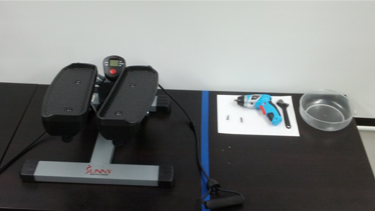
\includegraphics[width=\columnwidth]{fig/equipment.png}
    \caption{The piece of exercise equipment and tools we used in the task to create our dataset.}
    \label{fig:equipment}
    %\vspace{-16pt}
\end{figure}

The piece of exercise equipment we used for our task is shown on the left in Figure~\ref{fig:equipment} with the necessary tools shown on the right. The complete disassembly, photographing, and reassembly task consists of 66 actions. However, we used only the first eight actions of the disassembly portion of the task in our dataset. This task therefore consisted of 1) removing an electronic display, 2 and 3) removing two resistance cords, 4) attaching the proper drill bit to an electronic screwdriver, 5 and 6) removing the two steps, 7) unscrewing by hand a resistance knob, and 8) detaching a wheel. This task involves a mixture of tool use and hand manipulation of components of a variety of parts on the exercise device. It therefore requires a large amount of participant mobility.

For the data collection, each participant executed the disassembly procedure with the instructions for the procedure delivered via a prototype task support system developed on the Google Glass\footnote{\href{http://en.wikipedia.org/wiki/Google_Glass}{http://en.wikipedia.org/wiki/Google\_Glass}} Platform, a lightweight head-mounted display device. These types of task guidance systems are being developed in other work, but this system provides a good platform for the acquisition of egocentric video information captured from the Glass device's camera, so it was selected for this purpose. The device was modified slightly to better capture the salient visual content of the task execution. The modified device is shown in Figure~\ref{fig:glass}. We attached a mirror  at an angle of approximately 25$\degree$ from level to the device with a 3D printed mount. When manipulating objects with the hands in front of themselves, most people both tilt their heads downward slightly and look downward with their eyes. The head-mounted camera will move with the head tilt, and the mirror helps to correct for the additional downward direction contributed by eye movements. A sample frame captured from the egocentric camera and mirror during the task is shown in Figure~\ref{fig:TODOframe}.

\begin{figure}[!b]
    \centering
    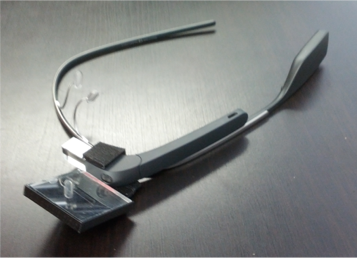
\includegraphics[width=\columnwidth]{fig/glass.png}
    \caption{The modified Google Glass device we used to capture the video for our dataset. The attached mirror helps to capture manipulations of objects directly in front of the procedure executor.}
    \label{fig:glass}
    %\vspace{-16pt}
\end{figure}

Each of the authors executed the eight actions of the exercise procedure ten times, resulting in our dataset of 30 egocentric videos of the same task. The authors had varying degrees of prior knowledge of the procedure, so the data consists of procedure executors of multiple levels of skill, resulting in a variety of techniques and times needed to execute the procedure. For example, one author had no knowledge of the procedure, and therefore initially relied completely on the task guidance delivered by the Glass device to preform the procedure. By the end of his tenth execution, he had internalized the procedure, eliminating the need for the assistance device, and was significantly faster than before. His set of ten videos, therefore, has him performing at a continuum of expertise levels as he increased in familiarity with the procedure. Thus, while there were only three participants included in the dataset, we believe there is still ample variety in the dataset and that testing with this data will generalize to other executors of the same procedure. Each of the actions in the video was segmented by hand to use for training and testing purposes in the classification.

\subsection{Results}

We evaluated our pipeline in a number of experiments using our exercise equipment disassembly dataset. In the following paragraphs we discuss the methodology used in our grid search of the pipeline parameters and the resulting accuracies.

We performed a grid search manipulating the following parameters: 1) the number of bins used in the HOOF histogram binning, 2) the size of the the codebook of HOOF features, and 3) the number of states in the HMMs. To evaluate each parameter configuration, we used a leave-one-out cross validation technique where 29 of the 30 videos were used to generate the codebook and train the HMMs. The actions of the last video were then each passed through the pipeline and the predicted action was the one which had the highest probability from the set of HMMs. The results using the Petri Network of the task used a weighting factor of 0.98. In all cases, random number generation was seeded such that k-means and the HMMs will produce repeatable results. Additionally, both of these processes were run with enough iterations to ensure convergence. To evaluate the accuracies of predicting each action for each configuration, we averaged (by action) these 30 accuracy results to determine a configuration accuracy. The results for some of the parameter configurations are shown in Table~\ref{tab:results}.
 
%\begin{table}[!tp]
%	\centering
%	\includegraphics[width=\columnwidth]{figures/TODO.JPG}
%	\caption{TODO Configuration accuracy results for each action for a subset of the grid search.}
%	\label{tab:results}
%\end{table}

While these accuracies are not spectacular, they are still significant in that random chance would put the accuracy at 0.125. Additionally, these results are comparable to accuracies in prior work that also use an egocentric camera~\cite{TODO-RONAK}. In the next section we discuss the challenges we discovered with our technique and the implications for future methods to improve the results of real-time prediction of actions from egocentric cameras.

\section{Discussion and Future Work}

While we were able to see the results of our pipeline, we expect there may be strong reasons for which our classification accuracy is not high. Due to time limitations, we were not able to further explore these issues, but they may prove to be valuable as future work.

\subsection{Diversity and Quantity of Training Data}

Though we were able to simulate the training data that may be obtained in an actual application of our work, during our testing we found misclassification issues that could be directly attributed to our training data. In many cases, the cluster sequences chosen for a particular test action were completely dissimilar to sequences that that action's HMM was trained on. While in a real-world streamed-data setting we might expect this, in our controlled experiment it seems to indicate our model is very susceptible to slight variations.

For this reason, we think our training data may be too similar. More diverse training data may allow for less overfitting, and create looser feature-cluster associations. In the same vein we note the small size of our dataset. Because of the requirement that we have a formal model of the activity being performed, we were required to create our own. Many learning methods require a large amount of data to create accurate predictions. Future work might include expanding and diversifying the training data, in a way that will allow the learning models to better generalize from training to testing.

\subsection{Low-Level Feature Representation}

While results from using Histograms of Optical Flow have been significant in the previous work cited above, we were not able to reach similar results even when attempting a one-vs.-all classification for each action. While the training data limitations would affect this, we expect an issue with our feature representation.

In our unique setup with an egocentric camera, we found that head movement tends to dominate any flow features found within the scene itself. Head movement was not controlled for at all during data acquisition, and as such head movement varied significantly across actions and across videos. Because these flows were primarily capturing this movement, we may have been learning models for head movement rather than the action in the scene.

For this reason we expect more work needs to be done in feature extraction in this domain. Theoretically our learning methods are sound, and given the right representation we expect much higher results. Some work has been done by Fathi et al.~\cite{fathi2011understanding} in the realm of egocentric video, but their implementations prove to be too slow for our activity guidance task. Future work might include incorporating object detection into the model, and using only the flow of tracked objects. Background subtraction and head movement compensation could also be explored as a means to increase the signal of the scene relative to head movement.
 
\section{Conclusion}



{\small
\bibliographystyle{ieee}
\bibliography{CS766_final_report}
}


\end{document}
